% Chapter Template

\chapter{Results} % Main chapter title

\label{Chapter3} % Change X to a consecutive number; for referencing this chapter elsewhere, use \ref{ChapterX}

%-------------------------------------------------------------------------------------
%	SECTION 1
%-------------------------------------------------------------------------------------
\section{Definition of error}
To assess the degree to which changes in the analysis pipeline affect the quality of measurement, a definition of error must first be decided upon. Because intensity varies so dramatically across the pharynx, we are interested in the amount of error \textit{relative} to the intensity at a particular location. Percent error ($\epsilon$) is defined to be a function over pharynx space ($p$) which is the difference between the intensity ($I$) measured in one frame and another, normalized by the average intensity of the two frames at a given wavelength, multiplied by 100. Thus, for $\lambda = 410\text{ nm}$, percent error is given by:

\[\epsilon(p) = \frac{|I_{410_1}(p) - I_{410_2}(p)|}{\frac{I_{410_1}(p) + I_{410_2}(p)}{2}} \times 100\]

% To calculate redox potentials, we take the first frame at 410 nm and the second at 470 nm. When we quantify error, however, we must use a single wavelength as the changes in emission spectra would confound the errors.


%-------------------------------------------------------------------------------------
%	SECTION 2
%-------------------------------------------------------------------------------------
\section{Collection of test data and baseline error quantification} \label{testCollection}

A large number of technical replicates were collected in order to establish a baseline empirical estimation of error. A single animal was imaged 57 times in pairs of two, both frames at 410 nm. The ratio images were hand-classified according to the degree of movement (see Figure \ref{fig:HighMovement}) in four regions: the posterior bulb, anterior bulb, sides of the tip, and tip. 
Figure \ref{fig:ErrorInOldPipeline} shows the average emperical error as a function of pharynx space, using the previous pipeline to estimate midlines and measure pixel intensities. At the boundaries of the pharynx, errors approach 75\% of the intensity, while errors are maximally around 10\% of the intensity in the interior regions of the pharynx. In animals that move, error tends to be larger, supporting the suggestion that inter-frame movement is a large source of error. Even in animals that do not move, errors can still reach 8\% in the interior regions of the  pharynx and increase dramatically at the boundaries.

% A paired-sample t-test indicates no significant difference (p=0.41) between the first and second intensity profile.

\begin{figure}
    \centering
    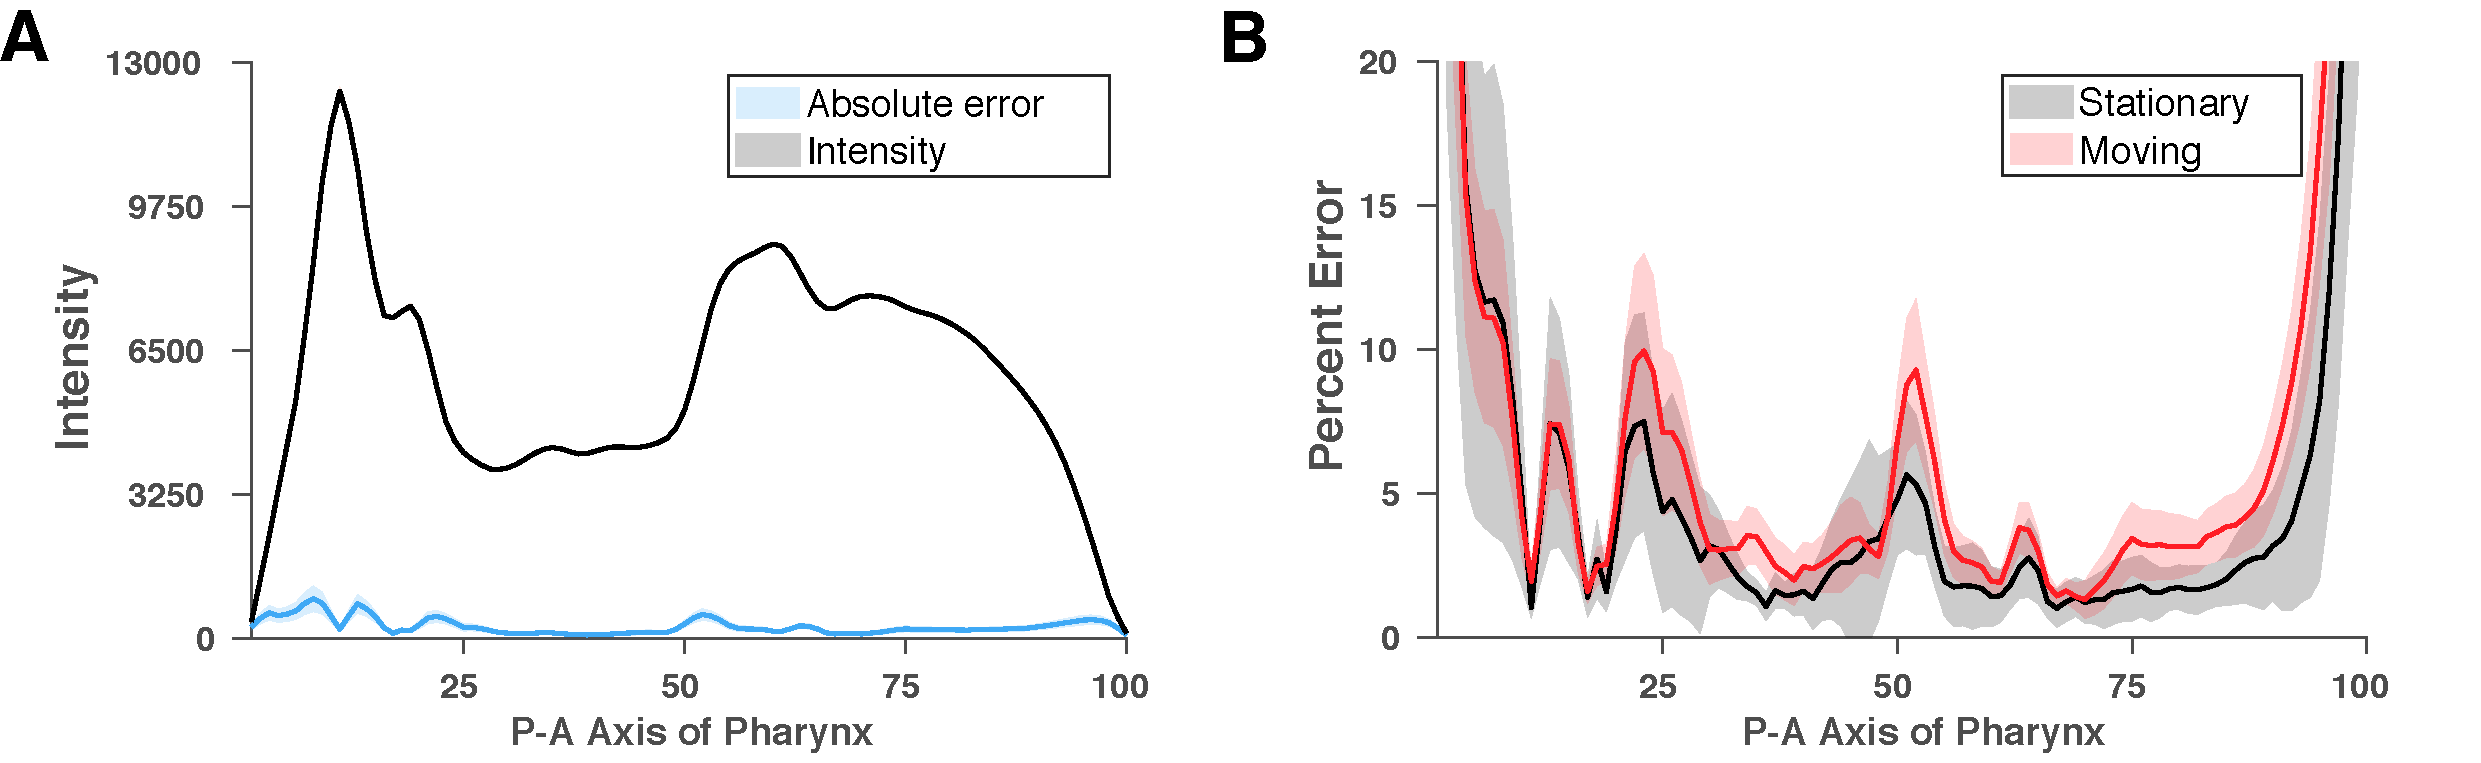
\includegraphics[scale=0.30]{Figures/rendered_files/error_and_intensity}
    \decoRule
    \caption[Errors in old pipeline]{Baseline quantification of empirical error in test data set. \textbf{A} shows the mean intensity (black) profile and absolute error (blue). Absolute error is defined as $|I_{410_1}(p)-I_{410_2}(p)|$. \textbf{B} shows the percent error in stationary (black) and moving (red) animals.}
    \label{fig:ErrorInOldPipeline}
\end{figure}

%-------------------------------------------------------------------------------------
%	SECTION 3
%-------------------------------------------------------------------------------------
% \section{A partially synthetic data set increases statistical power}

% Because each image in the test set is taken of the same animal, we can compare all possible pairs of images, instead of just those taken back-to-back. Given n images, we generate ${n \choose 2} = \frac{n!}{2!(n-2)!}$ pairs. However, repeated excitation seems to attenuate the total fluorescence of the sensors (Figure \ref{fig:AvgIntensityOverTime})\footnote{More biological replicates are needed to know if this effect is a general phenomenon or particular to this animal}. To account for this effect (known as photobleaching) we generate pairs starting after maximum photobleaching has occurred (by visual inspection) and exclude outliers (Figure \ref{fig:AvgIntensityOverTime}). After exclusion, this process generates 2,192 \todo{get real number} pairs of intensity profiles. This data set will be referred to as "synthetic", while the original will be referred to as "natural".

% \begin{figure}[ht]
%     \centering
%     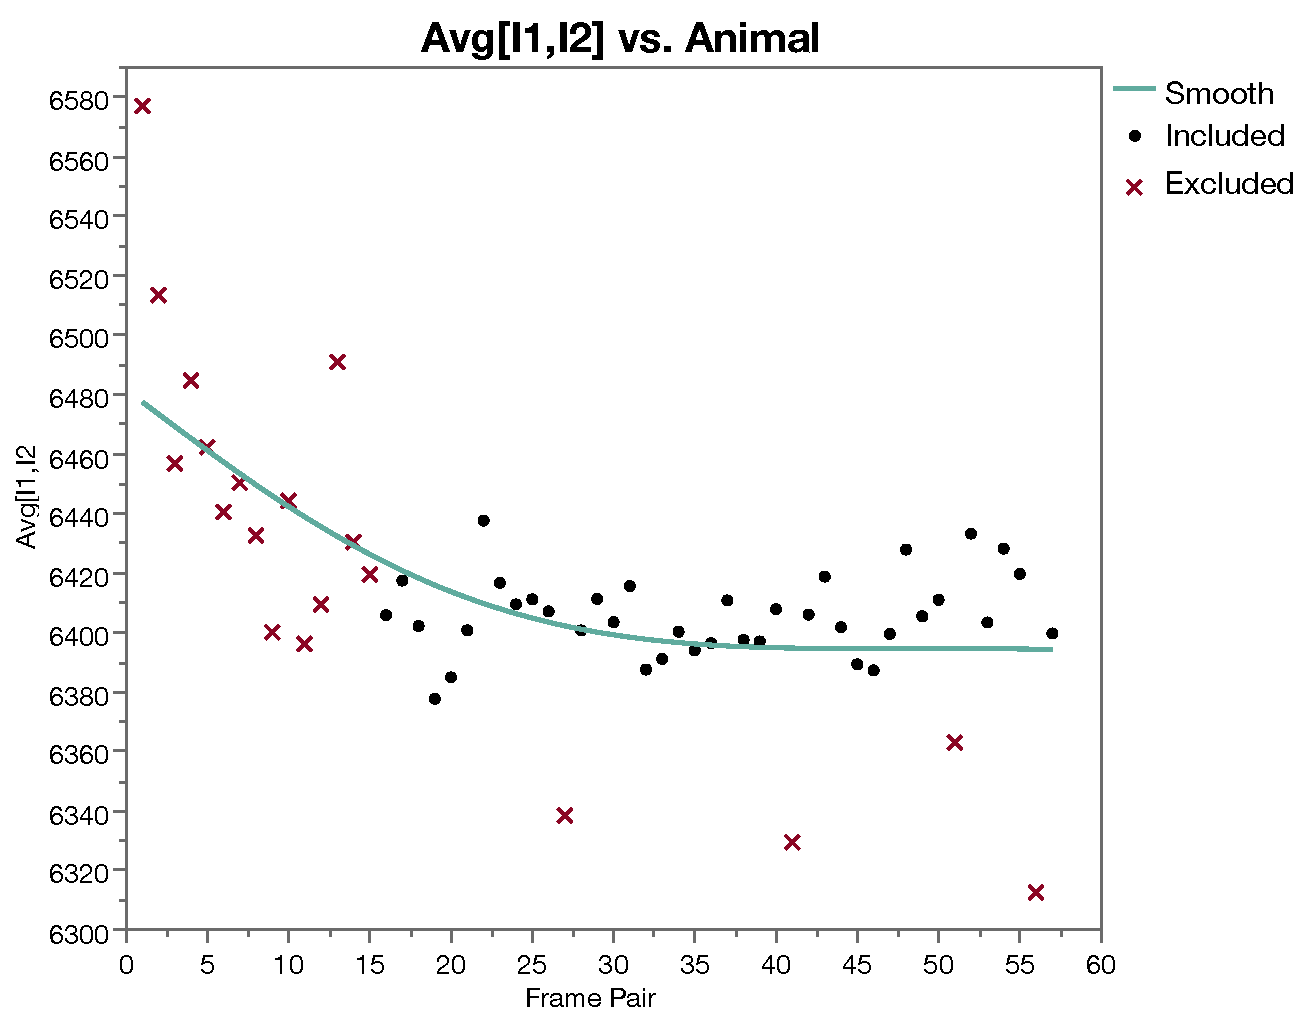
\includegraphics[scale=0.35]{Figures/rendered_files/photobleaching}
%     \decoRule
%     \caption[Average intensity over time in technical replicates]{The average intensity over time in technical replicates. Red xs mark image pairs excluded from the recombination.}
%     \label{fig:AvgIntensityOverTime}
% \end{figure}

% The long average time between pairs in the synthetic data results in a large degree of inter-frame movement. While inter-frame movement is generally undeseriable, it is useful to artificially generate it to study the effect it has on measurement error. A drawback of the synthetic data set is the large scale precludes manual movement annotation, and changes in error cannot be stratified by degree of movement.

%-------------------------------------------------------------------------------------
%	SECTION 4
%-------------------------------------------------------------------------------------
% \section{Reductions in manual intervention}

% \subsection{Incorporation of edge information increases segmentation accuracy}

% To compare the accuracy of segmentation methods, we first create a "gold-standard" set of images which were segmented by hand to ensure accuracy. The segmentation methods were applied to the same set of images and the resultant masks were compared via the total difference measure described in Yang et al. (A Supervised Approach to the Evaluation of Image Segmentation Methods).

% \todo[inline]{show figures comparing \% requiring manual intervention for segmentation and for midlines}

% \subsection{Incorporation of transmitted-light information increases centerline stability around the posterior bulb}

% To compare the stability of the centerline around the posterior bulb, we 

%-------------------------------------------------------------------------------------
%	SECTION 5
%-------------------------------------------------------------------------------------
\section{The new analysis pipeline reduces error}

The methods described in this thesis have a substantial effect on measurement error. The combined use of frame-specific masks/midlines and channel registration decreases error from ~3-9\% to less than 3\% across the entire pharynx (Figure \ref{fig:PercentErrorByStrategy}). Notably, the error around the boundaries remains stable when measuring with the new pipeline. The new pipeline decreases error across all regions of the pharynx, even in stationary animals.

\begin{figure}[ht]
    \centering
    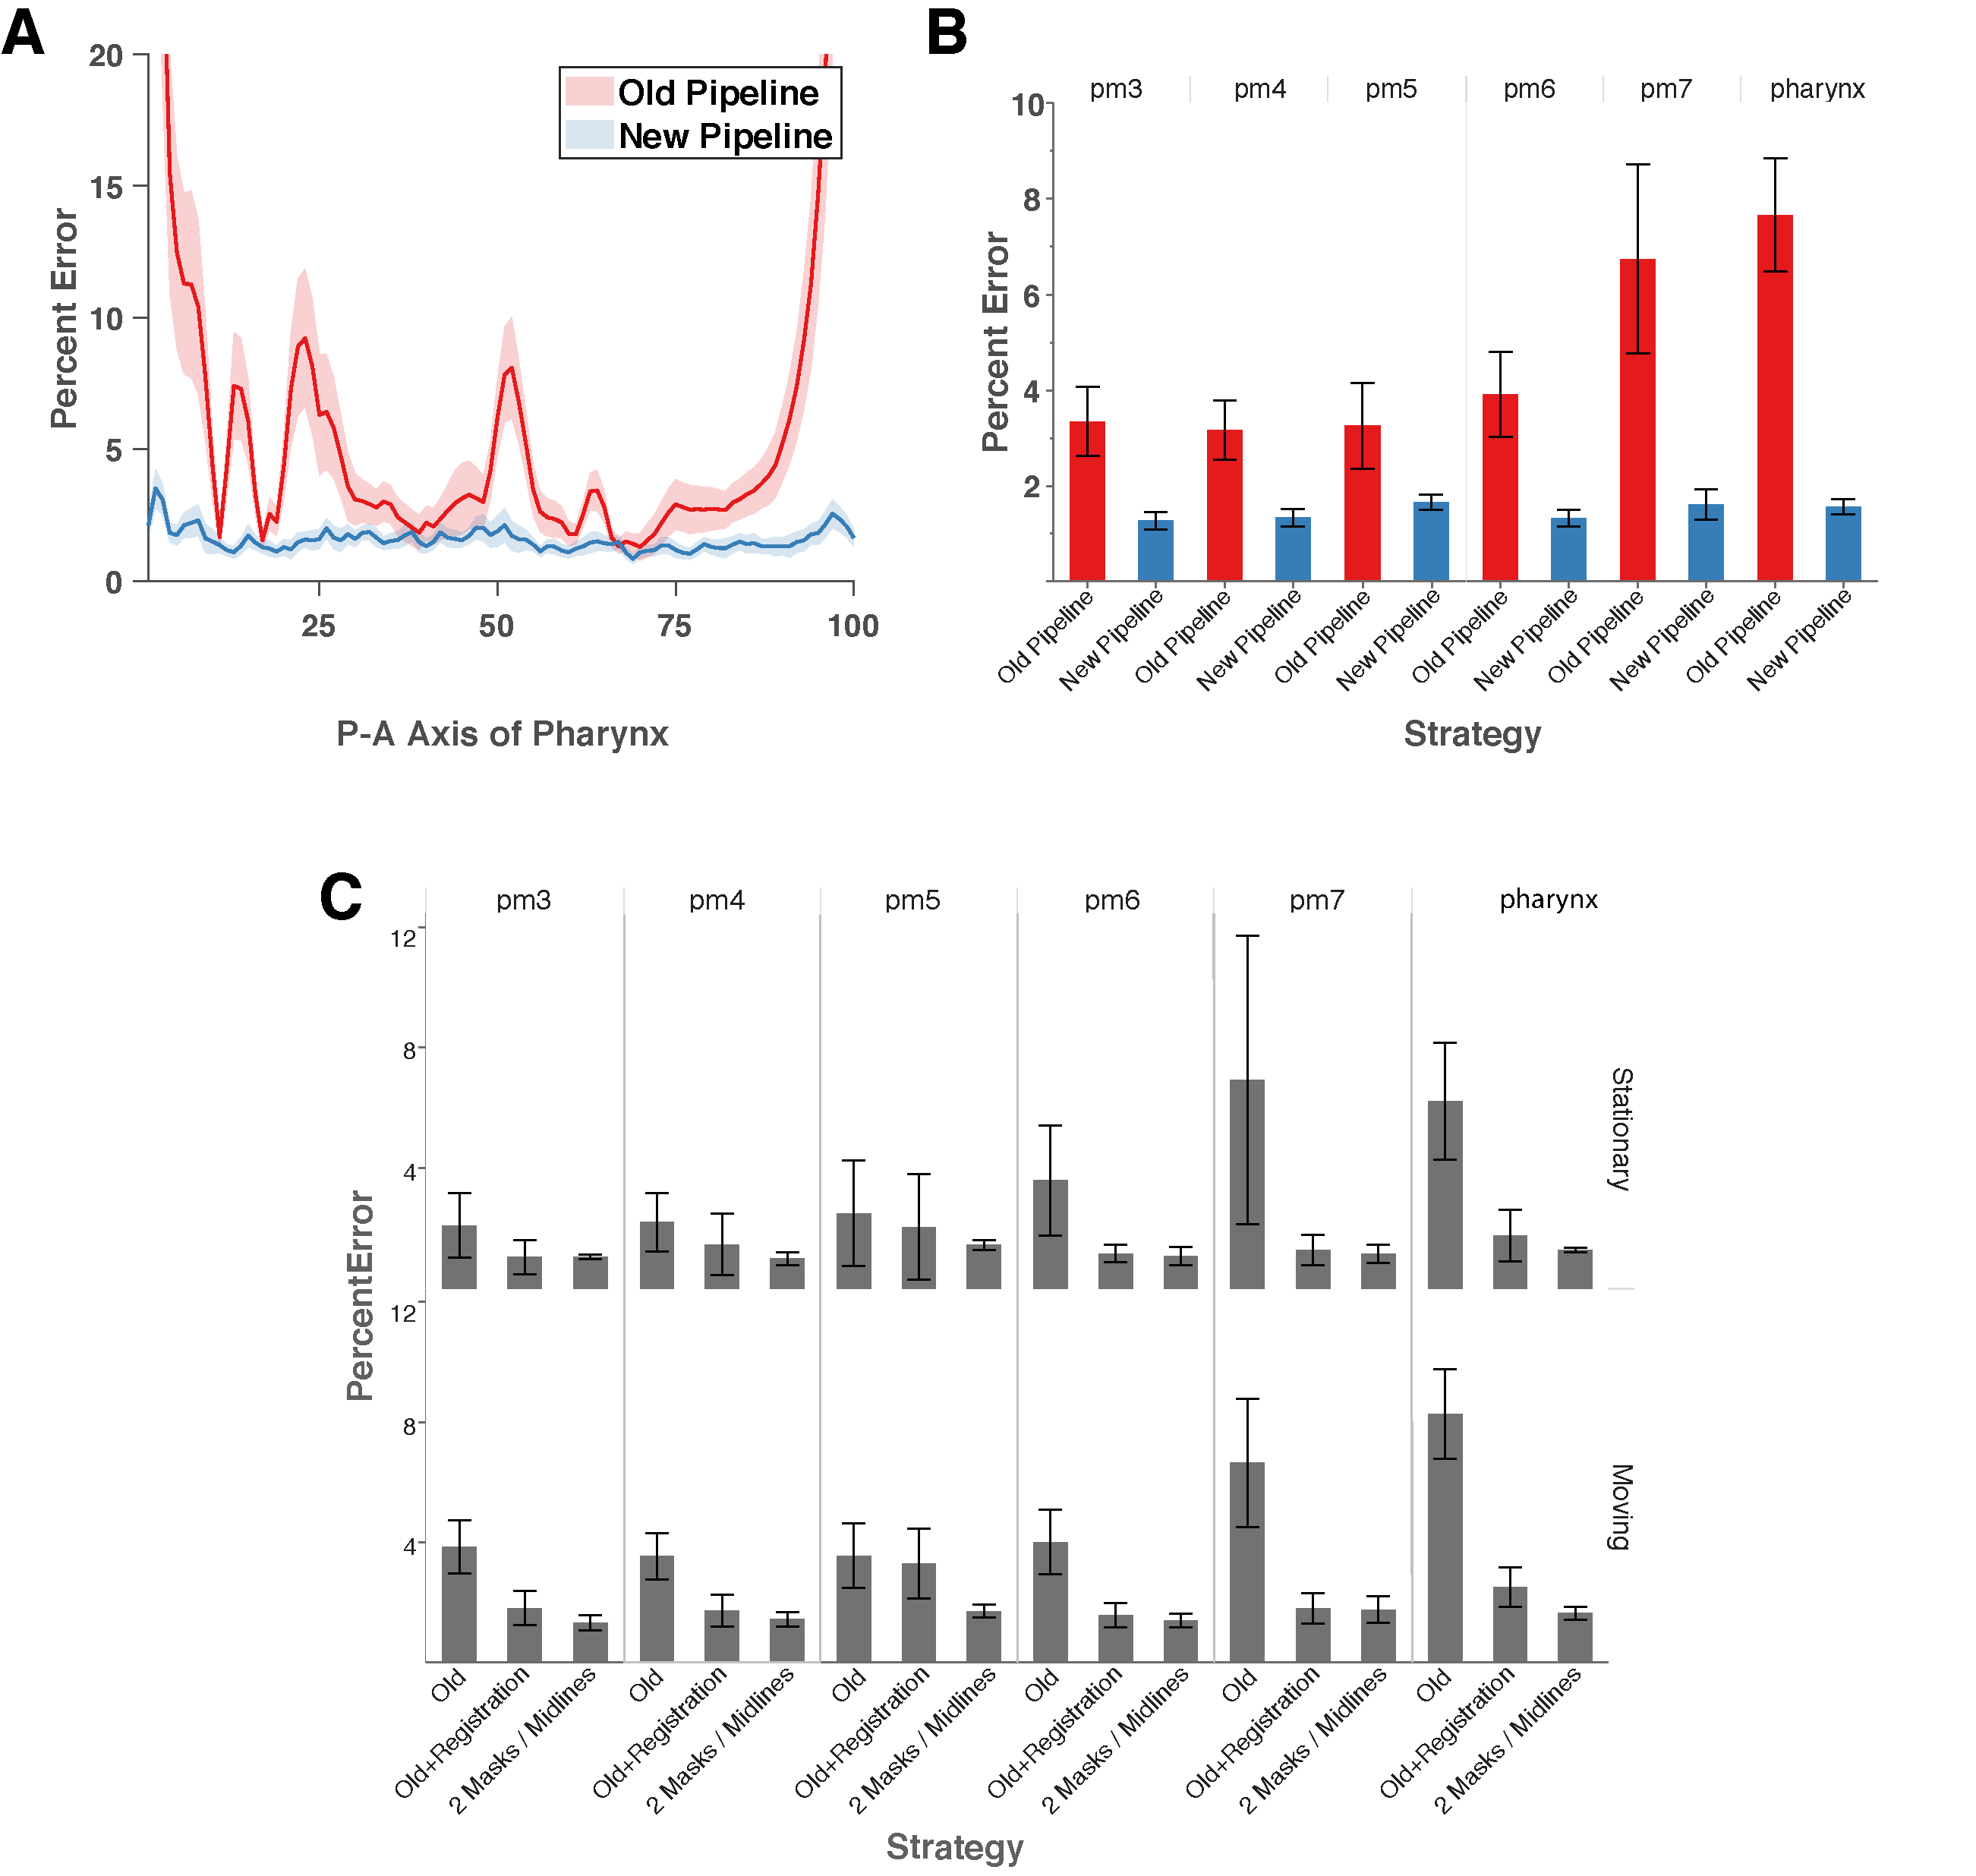
\includegraphics[scale=0.3]{Figures/rendered_files/errors_by_strategy}
    \decoRule
    \caption[Error by strategy in the synthetic data set]{\textbf{A} Percent error is reduced across the entire pharynx space by use of the new pipeline as compared to the old pipeline. \textbf{B} Errors are averaged over physiologically relevant boundaries. pm3--pm7 are cells in the pharyngeal muscle ordered sequentially along the posterior-anterior axis; "pharynx" refers to an average over the entire profile. \textbf{C} The effect of different strategies on percent error in stationary and moving animals. "Old+registration" applies the functional registration strategy described in \ref{method:Registration} to the intensity profiles obtained via the old pipeline, while "2 Masks / Midlines" uses the new methodologies for computing frame-specific masks and midlines but forgoes functional registration}
    \label{fig:PercentErrorByStrategy}
\end{figure}

Registration and frame-specific masks/midlines seem to act redundantly in reducing error. In effect, the flexible measurement boundaries enabled by frame-specific masks and midlines perform a limited form of registration. Specifically, they can register intensity profiles which need a linear stretch or compression (when the animal pumps between frames). When the pharynx moves dorsoventrally, the posterior regions of the pharynx remain stationary while the anterior tip of the pharynx moves. While a frame-specific midline can capture this movement, differences in the arc-length of the midline requires the non-linear registration strategy described in \ref{method:Registration}. Dorsoventral movement is relatively rare as compared to pumping, and a larger data set is needed to understand the quantitative reduction in error attributed to this non-linear registration.